\section{Anmelden und Navigieren}

\subsection{Anmeldebildschirm}

Ist die Installation gem�� Abschnitt \ref{sect:install} erfolgreich abgeschlossen, erscheint nach Aufruf der entsprechenden Adresse im Internetzugangsprogramm der \ATFROGSnosp-Anmeldebildschirm wie in Abbildung \ref{img:login} dargestellt.\\

\begin{figure}[htp]
   \centering
   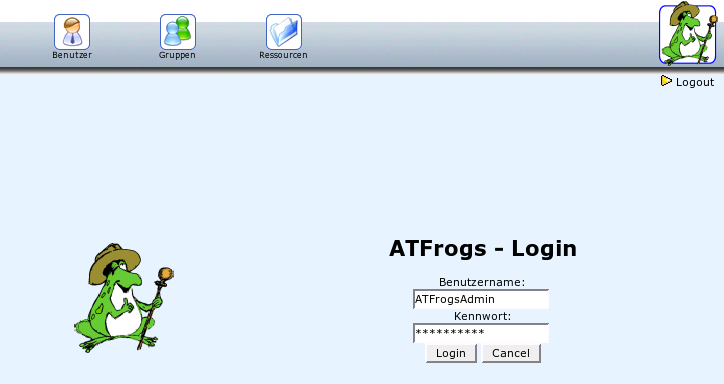
\includegraphics[width=\textwidth]{graphics/login}
   \caption{\ATFROGSnosp-Anmeldebildschirm}
   \label{img:login}
\end{figure}

Berechtigte Nutzer k�nnen sich nun an der Administrationsoberfl�che mit ihrem Benutzernamen und Kennwort anmelden. Ist die Anmeldung erfolgreich, gelangt man in die Ansicht einer der drei Module -- Benutzer, Gruppen oder Ressourcen (vgl. Abschnitt \ref{sect:install:editweb.xml}). Ist die Kombination von Benutzername und Kennwort falsch, so erscheint das Fenster erneut und die Eingabe kann korrigiert werden. \\

\subsection{Navigieren zwischen den Modulen}
Mit Hilfe der in Abbildung \ref{img:top_navigation} dargestellten Navigationsleiste, die sich in der Kopfzeile jedes Bildschirms befindet, l�sst sich bequem zwischen den drei \ATFROGSnosp-Modulen wechseln.

\begin{figure}[htp]
   \centering
   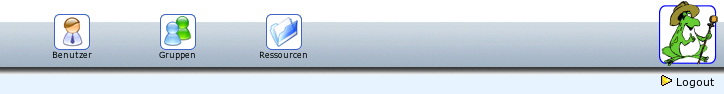
\includegraphics[width=\textwidth]{graphics/top_navigation}
   \caption{Navigationsleiste}
   \label{img:top_navigation}
\end{figure} 

\pagebreak
Die Navigationsleiste enth�lt die Symbole zum Zugriff auf die einzelnen \ATFROGSnosp-Module:


\begin{description}
\item[
\includegraphics{graphics/userlogo.png} Benutzeradministration]\

Durch einen Klick auf das Icon gelangt man in das Modul zur Benutzeradministration. Die Funktionen dieses Moduls werden in Kapitel \ref{sect:useradministration} dargestellt.
\item[
\includegraphics{graphics/grouplogo.png} Gruppenadministration]\

Durch einen Klick auf das Icon gelangt man in das Modul zur Gruppenadministration. Die Funktionen dieses Moduls werden in Kapitel \ref{sect:groupadministration} dargestellt.
\item[
\includegraphics{graphics/resourcelogo.png} Ressourcenadministration]\

Durch einen Klick auf das Icon gelangt man in das Modul zur Ressourcenadmi- nistration. Die Funktionen dieses Moduls werden in Kapitel \ref{sect:resourceadministration} dargestellt.
\end{description} \

Durch einen Klick auf 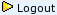
\includegraphics[scale=0.8]{graphics/logout.png} wird die aktuelle \ATFROGSnosp-Sitzung beendet. Wird diese Schaltfl�che gew�hlt, hat sich der Benutzer abgemeldet. Eine erneute Anmeldung vor der n�chsten Nutzung ist n�tig.\\

\NOTE{
Um unbefugte Zugriffe zu verhindern, sollte eine \ATFROGSnosp-Sitzung stets durch einen Klick auf 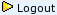
\includegraphics[scale=0.8]{graphics/logout.png} beendet werden!
}

\subsection{Einsehen der Konsolenausgabe}

Nach dem Durchf�hren einer Operation, die durch Ausf�hren eines der \OPENXCHANGE-Administrationsskripte realisiert wird, wird deren Konsolenausgabe in dem in Abbildung \ref{img:consoleOut} zu sehenden Textfeld unterhalb der Seite eingeblendet. 


\begin{figure}[htp]
   \centering
   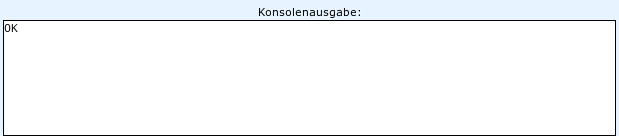
\includegraphics[width=\textwidth]{graphics/console_out}
   \caption{Anzeige der Konsolenausgabe}
   \label{img:consoleOut}
\end{figure} 



